After reviewing the different mechanisms by which an antibody aiming at
an antigen can lead to its elimination by the immune system, we are going
to study commercial products that uses monoclonal antibodies to fight
against cancers and viruses.

As it has already been noted, the mAbs serve as a precise means of targeting
specifically a cell or agent that will be treated naturally by the immune system ; 
the mAbs do not suppress any antigen on their own.

\subsubsection{Trastuzumab against HER2-positive breast cancer}

\begin{figure}[H]
    \begin{minipage}{0.495\textwidth}
            \centering
            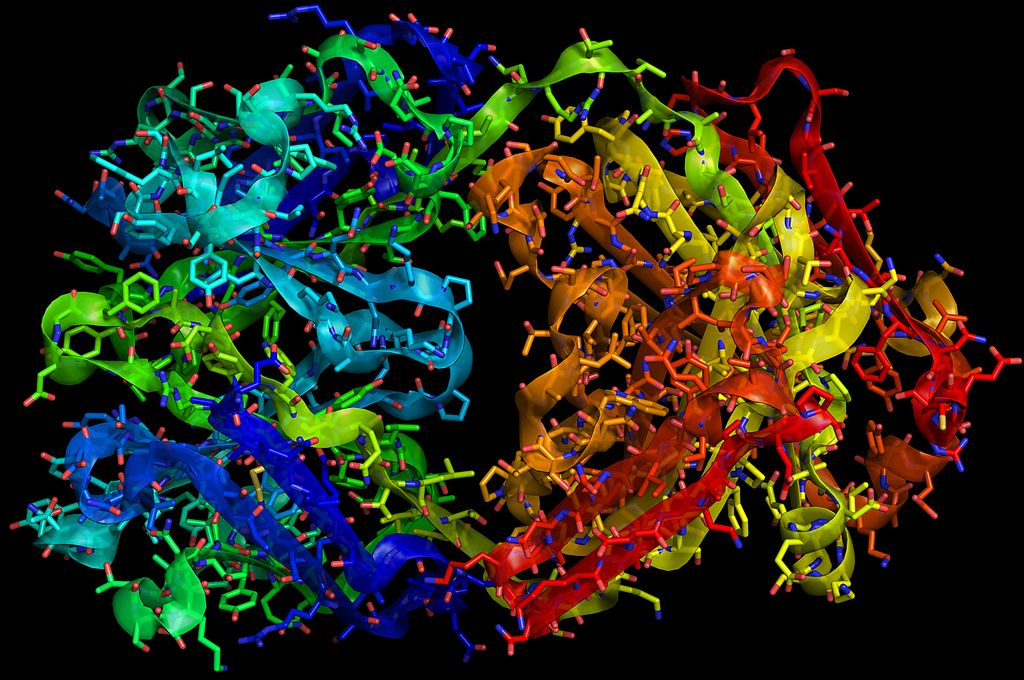
\includegraphics[width=\textwidth]{../Images/herceptin.jpg}
            \caption{Modelization of the trastuzumab molecule}
            \label{fig:trastuzumab}
    \end{minipage}\hfill
    \begin{minipage}{0.495\textwidth}
            \centering
            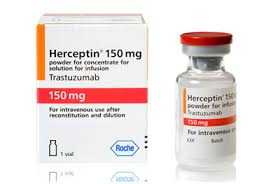
\includegraphics[width=\textwidth]{../Images/trastuzumab.jpg}
            \caption{Trastuzumab is sold by Roche under the name Herceptin
            \cite{roche_herceptin_nodate}}
            \label{fig:herceptin}
    \end{minipage}
\end{figure}

Breast cancer is one of the most common cancers in the world.
It concerns 25\% of cancer cases in women, with around 2 million new cases
each year. This type of cancer has thus been the target of many research efforts.

For a particular type of breast cancers called \emph{HER2 positive} (be it early 
or metastatic) which can be particularly aggressive, multiple treatments can
be considered. Surgery, radiation therapy can be used to remove part of the tumor ;
chemotherapy aims at treating chemically the cancer. However, these treatments are
not always fully effective at removing the tumor, especially for metastatic cancers,
were tumor cells travel in the bloodstream and fix themselves in another
part of the body.

\emph{Trastuzumab}, a humanized monoclonal antibody approved by the FDA in the 
United States in 1998, binds to a transmembrane protein called 
the \emph{HER2 receptor} \cite{zhao_trastuzumab_2021}. This protein is
overexpressed in 15 to 25 percent of breast cancers ; this overexpression
is linked with aggressive forms of the disease \cite{piccart-gebhart_trastuzumab_2005}.

Indeed, the proliferation of this protein at the surface of cells leads to their
uncontrolled multiplication, provoking the formation of a tumor.
Trastuzumab, by binding with the HER2 receptor, prevents its dimerization and
proliferation, and thus stops the growth of the cell.

It can by covalently associated with a cytotoxic called \emph{DM1} to form
\emph{trastuzumab emtansine}. This \emph{antibody-drug conjugate} (ADC) 
is associated with a higher disease-free survival rate
\cite{lambert_ado-trastuzumab_2014}.

Herceptin is delivered by injection over the course of one year.
It costs $17000$ € per patient. Herceptin can also be prescribed for treatment of stomach cancer. 
As this drug is comparatively old, multiple
biosimilars have been developed by concurrent laboratories. It used to be a
top-3 selling drug for Roche Pharma ; it brought a $6,08$ billion dollar
revenue in 2019 alone to the lab \cite{fierce_pharma_herceptin_2020}.


\subsubsection{Adalimumab against autoimmune diseases}
\begin{figure}[H]
    \begin{minipage}{0.49\textwidth}
            \centering
            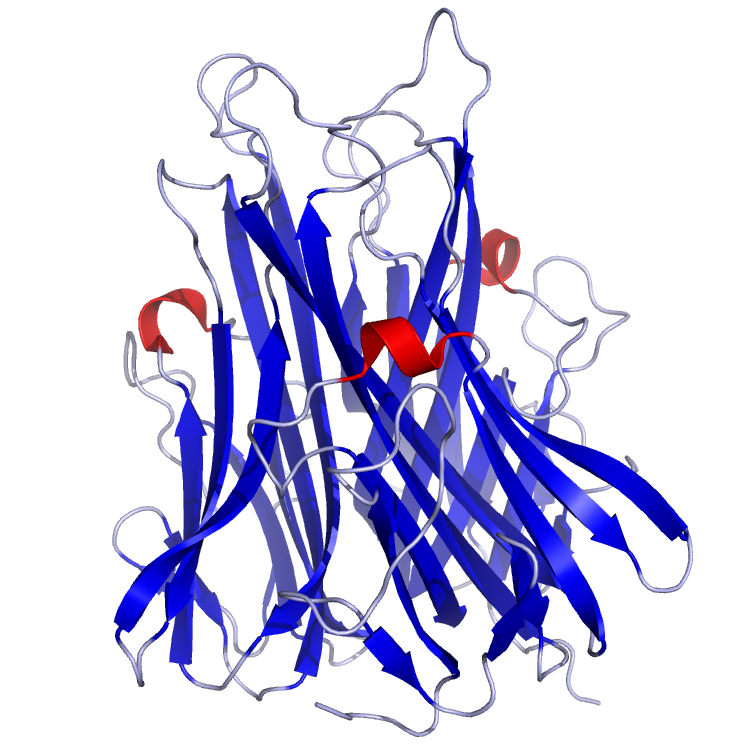
\includegraphics[width=0.6\textwidth]{../Images/TNFa_Crystal_Structure.rsh.png}
            \caption{Crystal structure of the TNF-$\alpha$ protein}
            \label{fig:TNFa_Crystal_Structure}
    \end{minipage}\hfill
    \begin{minipage}{0.49\textwidth}
            \centering
            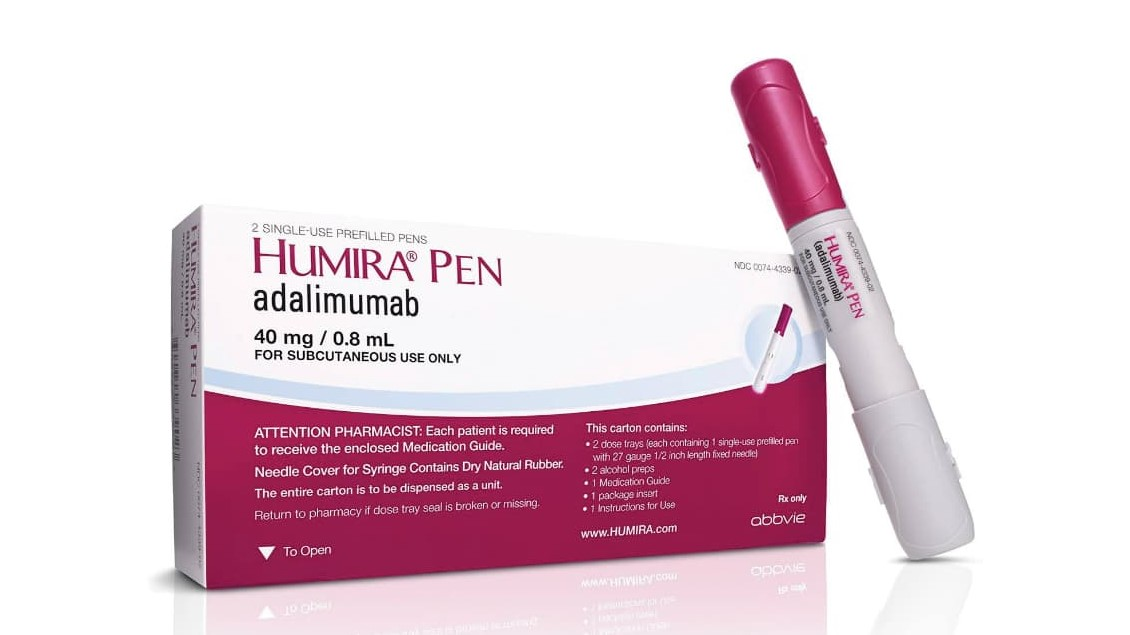
\includegraphics[width=\textwidth]{../Images/humira.jpg}   
            \caption{Adalimumab is sold by Abbvie under the name Humira \cite{noauthor_humira_nodate-1}}
            \label{fig:humira}
    \end{minipage}
\end{figure}

The \emph{Tumor Necrosis Factor-alpha} (TNF-$\alpha$) is a transmembrane protein
associated with the mechanism of inflammation. It helps recruiting lymphocytes
and macrophages to help locally fight pathogens.

However, it can be implicated in a number of autoimmune diseases including
ulcerative colitis, Crohn’s disease, plaque psoriasis, and arthritis
\cite{noauthor_adalimumab_2021}.

\emph{Adalimumab} is a fully human monoclonal antibody approved by the FDA in 2002.
This IgG$_1$ can bind to TNF-$\alpha$ and inhibit its activity, thus reducing the 
signs and symptoms in the diseases cited above, notably for rheumatoid arthritis
\cite{mease_adalimumab_2007}. It is delivered by subcutaneous injection, and mostly
prescribed to patients who have not responded well to previous treatments.

Humira (the drug based on this monoclonal antibody) has been for ten year
the world top-selling drug \cite{fierce_pharma_humira_2021}.
Being prescribed for treatment of rheumatoid arthritis, psoriatic arthritis and Crohn’s disease,
it grossed $20,39$ billion dollars in sales in 2020.


\subsubsection{Bebtelovimab (LY-CoV1404) against the SARS-CoV-2}
\begin{figure}[H]
    \begin{minipage}{0.49\textwidth}
        \centering
        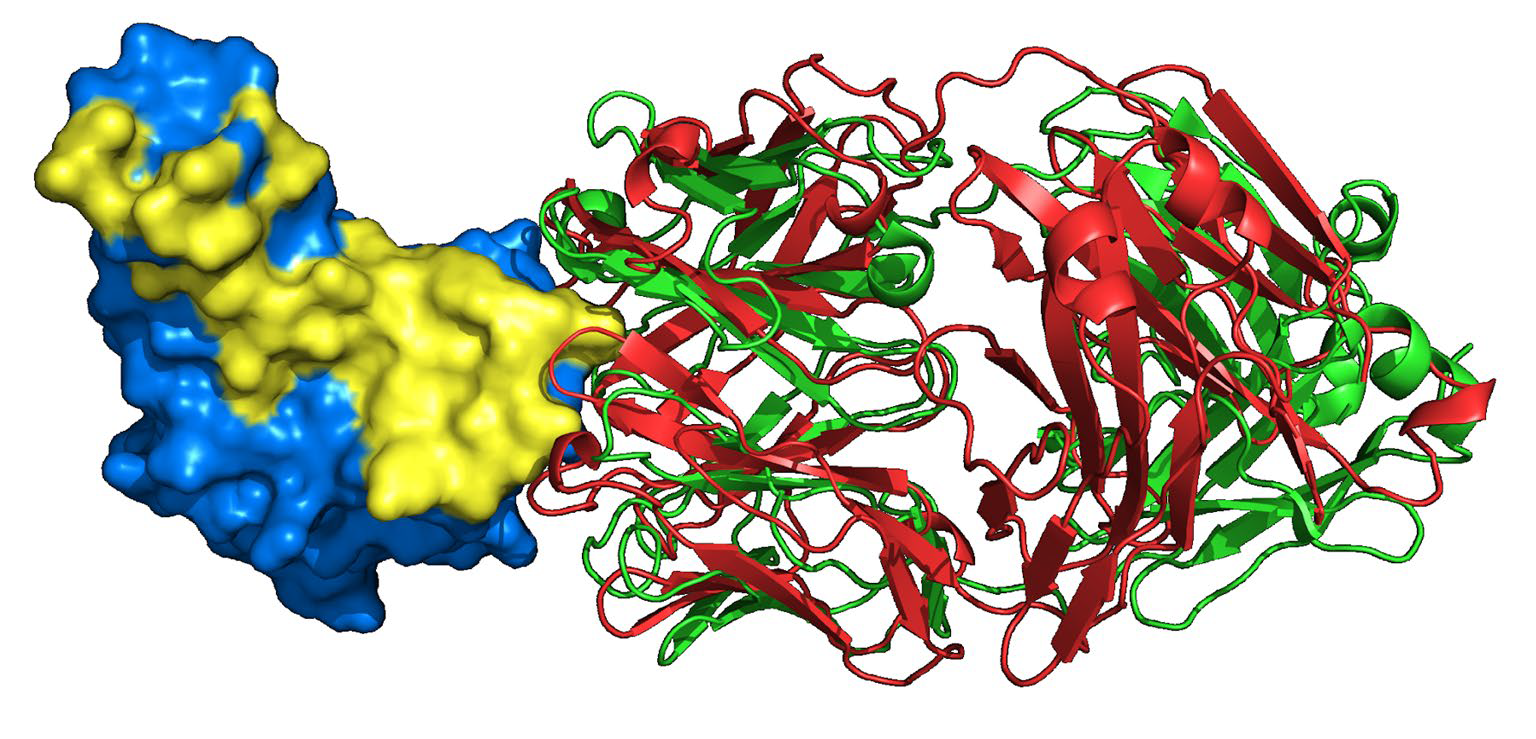
\includegraphics[width=\textwidth]{../Images/LY-CoV1404_spike_protein.png}
        \caption{LY-CoV1404 binds to the Spike protein RBD and blocks ACE2 interactions}
        \label{fig:LY-CoV1404_spike_protein}
    \end{minipage}\hfill
    \begin{minipage}{0.49\textwidth}
        \centering
        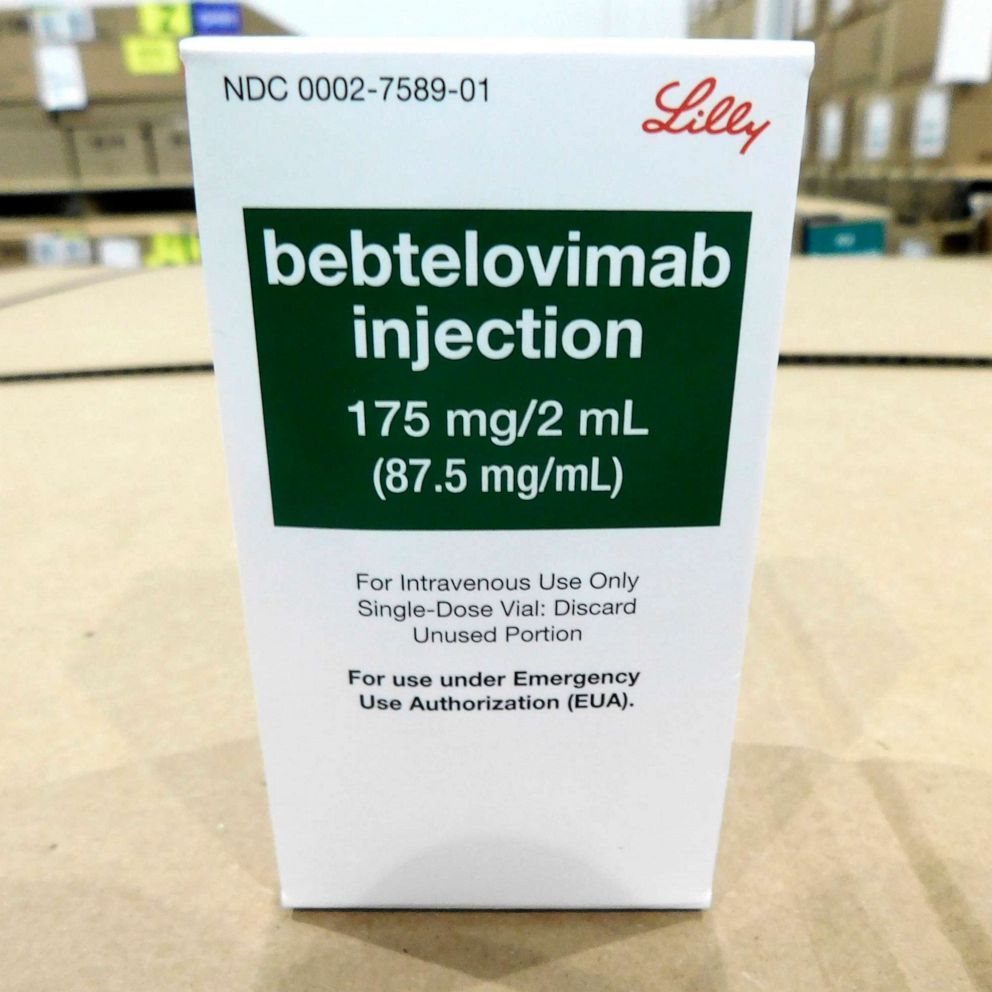
\includegraphics[width=0.5\textwidth]{../Images/bebtelovimab.jpg}   
        \caption{Bebtelovimab is used under a Emergency Use Authorization from the FDA}
        \label{fig:bebtelovimab}
    \end{minipage}
\end{figure}

Finally, we will discuss of some recent research targeting the SARS-CoV-2 pandemic
that emerged at the end of 2019 in China and spread worldwide quickly. Since then, there have
been more than $411$ million cases worldwide, leading to the death of more than $5,8$ million
people (as of February~17th 2022) \cite{noauthor_covid-19_nodate}.
This pandemic also led to major disruptions in the daily
life of many countries, with international travel being extremely restricted and entire 
countries placed under lockdown.

This encouraged heavy funding of research aiming at limiting the death toll of the
virus and its associated disease, COVID-19. Indeed, patients who were admitted to
Intensive Care Units (ICU) have to be treated for a very long time (around two weeks),
which leads to the quick saturation of these units, which are designed for short stays
\cite{mannucci_saturation_2020}.

One of the products resulting of this worldwide effort is \emph{bebtelovimab}, developed
by Eli Lilly and Company and subject to an Emergency Use Authorization (EUA)
by the FDA in February 2022 \cite{office_of_the_commissioner_coronavirus_2022}
\cite{eli_lilly_lillys_2022}. It aims at preventing people contaminated with
the virus, and who have a high probability of developing severe illness, from
being hospitalized and even from death. 

Bebtelovimab is a SARS-CoV-2 spike glycoprotein receptor binding domain
(RBD)-specific antibody. The spike protein is specific to SARS-CoV-2.
Also known as LY-CoV1404, this monoclonal antibody is highly potent because
the epitope it targets is rarely mutated, and it can thus neutralize all the
SARS-CoV-2 variants of concern that were identified across 
the globe \cite{westendorf_ly-cov1404_2022}. The viruses whose spike proteins
are bound to this antibody cannot infect human cells since they cannot attach
to the cell receptor they usually target \cite{wang_sars_2008}.
LY-CoV1404 is a fully human monoclonal antibody, that is produced from a clone
of a B-cell extracted from the blood of a patient who had been infected with
SARS-CoV-2 and recovered from COVID-19 \cite{westendorf_ly-cov1404_2022}.

Finally, we can recall that the US President Donald Trump, who was contaminated
with COVID-19, was treated with an experimental monoclonal antibody cocktail,
consisting of one human antibody and one humanized antibody \cite{cohen_update_2020}. 
This aimed at preventing him from developing a severe COVID-19 form, which did not occur.
